\documentclass[twoside]{book}

% Packages required by doxygen
\usepackage{calc}
\usepackage{doxygen}
\usepackage{graphicx}
\usepackage[utf8]{inputenc}
\usepackage{makeidx}
\usepackage{multicol}
\usepackage{multirow}
\usepackage{textcomp}
\usepackage[table]{xcolor}

% Font selection
\usepackage[T1]{fontenc}
\usepackage{mathptmx}
\usepackage[scaled=.90]{helvet}
\usepackage{courier}
\usepackage{amssymb}
\usepackage{sectsty}
\renewcommand{\familydefault}{\sfdefault}
\allsectionsfont{%
  \fontseries{bc}\selectfont%
  \color{darkgray}%
}
\renewcommand{\DoxyLabelFont}{%
  \fontseries{bc}\selectfont%
  \color{darkgray}%
}

% Page & text layout
\usepackage{geometry}
\geometry{%
  a4paper,%
  top=2.5cm,%
  bottom=2.5cm,%
  left=2.5cm,%
  right=2.5cm%
}
\tolerance=750
\hfuzz=15pt
\hbadness=750
\setlength{\emergencystretch}{15pt}
\setlength{\parindent}{0cm}
\setlength{\parskip}{0.2cm}
\makeatletter
\renewcommand{\paragraph}{%
  \@startsection{paragraph}{4}{0ex}{-1.0ex}{1.0ex}{%
    \normalfont\normalsize\bfseries\SS@parafont%
  }%
}
\renewcommand{\subparagraph}{%
  \@startsection{subparagraph}{5}{0ex}{-1.0ex}{1.0ex}{%
    \normalfont\normalsize\bfseries\SS@subparafont%
  }%
}
\makeatother

% Headers & footers
\usepackage{fancyhdr}
\pagestyle{fancyplain}
\fancyhead[LE]{\fancyplain{}{\bfseries\thepage}}
\fancyhead[CE]{\fancyplain{}{}}
\fancyhead[RE]{\fancyplain{}{\bfseries\leftmark}}
\fancyhead[LO]{\fancyplain{}{\bfseries\rightmark}}
\fancyhead[CO]{\fancyplain{}{}}
\fancyhead[RO]{\fancyplain{}{\bfseries\thepage}}
\fancyfoot[LE]{\fancyplain{}{}}
\fancyfoot[CE]{\fancyplain{}{}}
\fancyfoot[RE]{\fancyplain{}{\bfseries\scriptsize Generated on Mon Aug 19 2013 15:37:05 for nAnthill by Doxygen }}
\fancyfoot[LO]{\fancyplain{}{\bfseries\scriptsize Generated on Mon Aug 19 2013 15:37:05 for nAnthill by Doxygen }}
\fancyfoot[CO]{\fancyplain{}{}}
\fancyfoot[RO]{\fancyplain{}{}}
\renewcommand{\footrulewidth}{0.4pt}
\renewcommand{\chaptermark}[1]{%
  \markboth{#1}{}%
}
\renewcommand{\sectionmark}[1]{%
  \markright{\thesection\ #1}%
}

% Indices & bibliography
\usepackage{natbib}
\usepackage[titles]{tocloft}
\setcounter{tocdepth}{3}
\setcounter{secnumdepth}{5}
\makeindex

% Hyperlinks (required, but should be loaded last)
\usepackage{ifpdf}
\ifpdf
  \usepackage[pdftex,pagebackref=true]{hyperref}
\else
  \usepackage[ps2pdf,pagebackref=true]{hyperref}
\fi
\hypersetup{%
  colorlinks=true,%
  linkcolor=blue,%
  citecolor=blue,%
  unicode%
}

% Custom commands
\newcommand{\clearemptydoublepage}{%
  \newpage{\pagestyle{empty}\cleardoublepage}%
}


%===== C O N T E N T S =====

\begin{document}

% Titlepage & ToC
\hypersetup{pageanchor=false}
\pagenumbering{roman}
\begin{titlepage}
\vspace*{7cm}
\begin{center}%
{\Large n\-Anthill \\[1ex]\large x.\-y }\\
\vspace*{1cm}
{\large Generated by Doxygen 1.8.4}\\
\vspace*{0.5cm}
{\small Mon Aug 19 2013 15:37:05}\\
\end{center}
\end{titlepage}
\clearemptydoublepage
\tableofcontents
\clearemptydoublepage
\pagenumbering{arabic}
\hypersetup{pageanchor=true}

%--- Begin generated contents ---
\chapter{Hierarchical Index}
\section{Class Hierarchy}
This inheritance list is sorted roughly, but not completely, alphabetically\-:\begin{DoxyCompactList}
\item \contentsline{section}{Comm}{\pageref{classComm}}{}
\item \contentsline{section}{Message}{\pageref{classMessage}}{}
\item \contentsline{section}{Process}{\pageref{classProcess}}{}
\begin{DoxyCompactList}
\item \contentsline{section}{Manager}{\pageref{classManager}}{}
\item \contentsline{section}{Worker}{\pageref{classWorker}}{}
\end{DoxyCompactList}
\end{DoxyCompactList}

\chapter{Class Index}
\section{Class List}
Here are the classes, structs, unions and interfaces with brief descriptions\-:\begin{DoxyCompactList}
\item\contentsline{section}{\hyperlink{classComm}{Comm} }{\pageref{classComm}}{}
\item\contentsline{section}{\hyperlink{classManager}{Manager} }{\pageref{classManager}}{}
\item\contentsline{section}{\hyperlink{classMessage}{Message} }{\pageref{classMessage}}{}
\item\contentsline{section}{\hyperlink{classProcess}{Process} }{\pageref{classProcess}}{}
\item\contentsline{section}{\hyperlink{classWorker}{Worker} }{\pageref{classWorker}}{}
\end{DoxyCompactList}

\chapter{File Index}
\section{File List}
Here is a list of all files with brief descriptions\-:\begin{DoxyCompactList}
\item\contentsline{section}{comm/\hyperlink{comm_8hpp}{comm.\-hpp} }{\pageref{comm_8hpp}}{}
\item\contentsline{section}{manager/\hyperlink{manager_8cpp}{manager.\-cpp} }{\pageref{manager_8cpp}}{}
\item\contentsline{section}{manager/\hyperlink{manager_8hpp}{manager.\-hpp} }{\pageref{manager_8hpp}}{}
\item\contentsline{section}{process/\hyperlink{message_8cpp}{message.\-cpp} }{\pageref{message_8cpp}}{}
\item\contentsline{section}{process/\hyperlink{message_8hpp}{message.\-hpp} }{\pageref{message_8hpp}}{}
\item\contentsline{section}{process/\hyperlink{process_8hpp}{process.\-hpp} }{\pageref{process_8hpp}}{}
\item\contentsline{section}{worker/\hyperlink{worker_8cpp}{worker.\-cpp} }{\pageref{worker_8cpp}}{}
\item\contentsline{section}{worker/\hyperlink{worker_8hpp}{worker.\-hpp} }{\pageref{worker_8hpp}}{}
\end{DoxyCompactList}

\chapter{Class Documentation}
\hypertarget{classComm}{\section{Comm Class Reference}
\label{classComm}\index{Comm@{Comm}}
}


{\ttfamily \#include $<$comm.\-hpp$>$}

\subsection*{Protected Member Functions}
\begin{DoxyCompactItemize}
\item 
\hyperlink{classComm_a47668b629f7201a6ada3ff3afa4ff712}{Comm} ()
\item 
\hyperlink{classComm_a00134417af6aae9bf911d3ec7b8c049b}{$\sim$\-Comm} ()
\end{DoxyCompactItemize}


\subsection{Constructor \& Destructor Documentation}
\hypertarget{classComm_a47668b629f7201a6ada3ff3afa4ff712}{\index{Comm@{Comm}!Comm@{Comm}}
\index{Comm@{Comm}!Comm@{Comm}}
\subsubsection[{Comm}]{\setlength{\rightskip}{0pt plus 5cm}Comm\-::\-Comm (
\begin{DoxyParamCaption}
{}
\end{DoxyParamCaption}
)\hspace{0.3cm}{\ttfamily [inline]}, {\ttfamily [protected]}}}\label{classComm_a47668b629f7201a6ada3ff3afa4ff712}

\begin{DoxyCode}
18            \{
19     \}
\end{DoxyCode}
\hypertarget{classComm_a00134417af6aae9bf911d3ec7b8c049b}{\index{Comm@{Comm}!$\sim$\-Comm@{$\sim$\-Comm}}
\index{$\sim$\-Comm@{$\sim$\-Comm}!Comm@{Comm}}
\subsubsection[{$\sim$\-Comm}]{\setlength{\rightskip}{0pt plus 5cm}Comm\-::$\sim$\-Comm (
\begin{DoxyParamCaption}
{}
\end{DoxyParamCaption}
)\hspace{0.3cm}{\ttfamily [inline]}, {\ttfamily [protected]}}}\label{classComm_a00134417af6aae9bf911d3ec7b8c049b}

\begin{DoxyCode}
22             \{
23     \}
\end{DoxyCode}


The documentation for this class was generated from the following file\-:\begin{DoxyCompactItemize}
\item 
comm/\hyperlink{comm_8hpp}{comm.\-hpp}\end{DoxyCompactItemize}

\hypertarget{classManager}{\section{Manager Class Reference}
\label{classManager}\index{Manager@{Manager}}
}


{\ttfamily \#include $<$manager.\-hpp$>$}



Inheritance diagram for Manager\-:\nopagebreak
\begin{figure}[H]
\begin{center}
\leavevmode
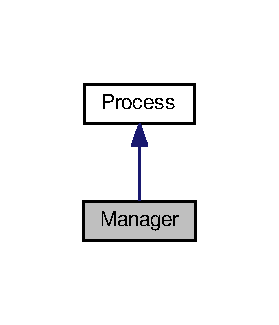
\includegraphics[width=134pt]{classManager__inherit__graph}
\end{center}
\end{figure}


Collaboration diagram for Manager\-:\nopagebreak
\begin{figure}[H]
\begin{center}
\leavevmode
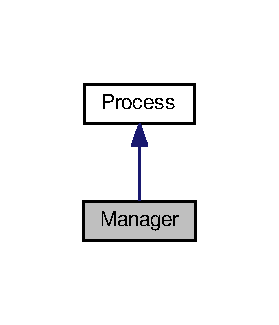
\includegraphics[width=134pt]{classManager__coll__graph}
\end{center}
\end{figure}
\subsection*{Public Member Functions}
\begin{DoxyCompactItemize}
\item 
\hyperlink{classManager_a1658ff9f18e38ccd9cb8b0b371b9c20b}{Manager} ()
\item 
\hyperlink{classManager_a322cad25d7007438b3a043ad02253d29}{$\sim$\-Manager} ()
\end{DoxyCompactItemize}
\subsection*{Additional Inherited Members}


\subsection{Constructor \& Destructor Documentation}
\hypertarget{classManager_a1658ff9f18e38ccd9cb8b0b371b9c20b}{\index{Manager@{Manager}!Manager@{Manager}}
\index{Manager@{Manager}!Manager@{Manager}}
\subsubsection[{Manager}]{\setlength{\rightskip}{0pt plus 5cm}Manager\-::\-Manager (
\begin{DoxyParamCaption}
{}
\end{DoxyParamCaption}
)\hspace{0.3cm}{\ttfamily [inline]}}}\label{classManager_a1658ff9f18e38ccd9cb8b0b371b9c20b}

\begin{DoxyCode}
25               \{
26     \}
\end{DoxyCode}
\hypertarget{classManager_a322cad25d7007438b3a043ad02253d29}{\index{Manager@{Manager}!$\sim$\-Manager@{$\sim$\-Manager}}
\index{$\sim$\-Manager@{$\sim$\-Manager}!Manager@{Manager}}
\subsubsection[{$\sim$\-Manager}]{\setlength{\rightskip}{0pt plus 5cm}Manager\-::$\sim$\-Manager (
\begin{DoxyParamCaption}
{}
\end{DoxyParamCaption}
)\hspace{0.3cm}{\ttfamily [inline]}}}\label{classManager_a322cad25d7007438b3a043ad02253d29}

\begin{DoxyCode}
29                \{
30     \}
\end{DoxyCode}


The documentation for this class was generated from the following file\-:\begin{DoxyCompactItemize}
\item 
manager/\hyperlink{manager_8hpp}{manager.\-hpp}\end{DoxyCompactItemize}

\hypertarget{classMessage}{\section{Message Class Reference}
\label{classMessage}\index{Message@{Message}}
}


{\ttfamily \#include $<$message.\-hpp$>$}

\subsection*{Public Member Functions}
\begin{DoxyCompactItemize}
\item 
\hyperlink{classMessage_a4fc4f717b634e66070366cb7722d7761}{Message} ()
\item 
\hyperlink{classMessage_a3f7275462831f787a861271687bcad67}{$\sim$\-Message} ()
\end{DoxyCompactItemize}


\subsection{Constructor \& Destructor Documentation}
\hypertarget{classMessage_a4fc4f717b634e66070366cb7722d7761}{\index{Message@{Message}!Message@{Message}}
\index{Message@{Message}!Message@{Message}}
\subsubsection[{Message}]{\setlength{\rightskip}{0pt plus 5cm}Message\-::\-Message (
\begin{DoxyParamCaption}
{}
\end{DoxyParamCaption}
)\hspace{0.3cm}{\ttfamily [inline]}}}\label{classMessage_a4fc4f717b634e66070366cb7722d7761}

\begin{DoxyCode}
19               \{
20     \}
\end{DoxyCode}
\hypertarget{classMessage_a3f7275462831f787a861271687bcad67}{\index{Message@{Message}!$\sim$\-Message@{$\sim$\-Message}}
\index{$\sim$\-Message@{$\sim$\-Message}!Message@{Message}}
\subsubsection[{$\sim$\-Message}]{\setlength{\rightskip}{0pt plus 5cm}Message\-::$\sim$\-Message (
\begin{DoxyParamCaption}
{}
\end{DoxyParamCaption}
)\hspace{0.3cm}{\ttfamily [inline]}}}\label{classMessage_a3f7275462831f787a861271687bcad67}

\begin{DoxyCode}
23                \{
24     \}
\end{DoxyCode}


The documentation for this class was generated from the following file\-:\begin{DoxyCompactItemize}
\item 
process/\hyperlink{message_8hpp}{message.\-hpp}\end{DoxyCompactItemize}

\hypertarget{classProcess}{\section{Process Class Reference}
\label{classProcess}\index{Process@{Process}}
}


{\ttfamily \#include $<$process.\-hpp$>$}



Inheritance diagram for Process\-:\nopagebreak
\begin{figure}[H]
\begin{center}
\leavevmode
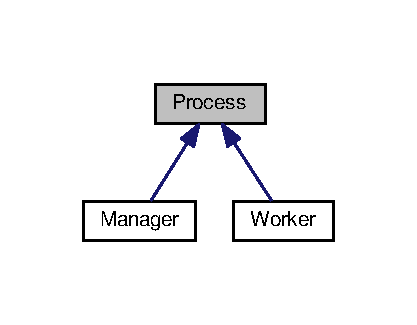
\includegraphics[width=200pt]{classProcess__inherit__graph}
\end{center}
\end{figure}
\subsection*{Protected Member Functions}
\begin{DoxyCompactItemize}
\item 
\hyperlink{classProcess_a9f4553eac74c657bb451f390c17d6bea}{Process} ()
\item 
\hyperlink{classProcess_a990776d181dbbde7ff8ac12713d814b3}{$\sim$\-Process} ()
\end{DoxyCompactItemize}


\subsection{Constructor \& Destructor Documentation}
\hypertarget{classProcess_a9f4553eac74c657bb451f390c17d6bea}{\index{Process@{Process}!Process@{Process}}
\index{Process@{Process}!Process@{Process}}
\subsubsection[{Process}]{\setlength{\rightskip}{0pt plus 5cm}Process\-::\-Process (
\begin{DoxyParamCaption}
{}
\end{DoxyParamCaption}
)\hspace{0.3cm}{\ttfamily [inline]}, {\ttfamily [protected]}}}\label{classProcess_a9f4553eac74c657bb451f390c17d6bea}

\begin{DoxyCode}
20               \{
21     \}
\end{DoxyCode}
\hypertarget{classProcess_a990776d181dbbde7ff8ac12713d814b3}{\index{Process@{Process}!$\sim$\-Process@{$\sim$\-Process}}
\index{$\sim$\-Process@{$\sim$\-Process}!Process@{Process}}
\subsubsection[{$\sim$\-Process}]{\setlength{\rightskip}{0pt plus 5cm}Process\-::$\sim$\-Process (
\begin{DoxyParamCaption}
{}
\end{DoxyParamCaption}
)\hspace{0.3cm}{\ttfamily [inline]}, {\ttfamily [protected]}}}\label{classProcess_a990776d181dbbde7ff8ac12713d814b3}

\begin{DoxyCode}
24                \{
25     \}
\end{DoxyCode}


The documentation for this class was generated from the following file\-:\begin{DoxyCompactItemize}
\item 
process/\hyperlink{process_8hpp}{process.\-hpp}\end{DoxyCompactItemize}

\hypertarget{classWorker}{\section{Worker Class Reference}
\label{classWorker}\index{Worker@{Worker}}
}


{\ttfamily \#include $<$worker.\-hpp$>$}



Inheritance diagram for Worker\-:\nopagebreak
\begin{figure}[H]
\begin{center}
\leavevmode
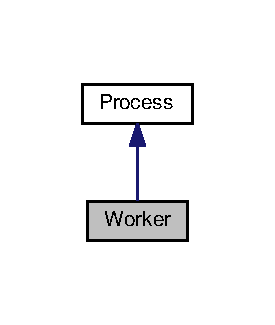
\includegraphics[width=132pt]{classWorker__inherit__graph}
\end{center}
\end{figure}


Collaboration diagram for Worker\-:\nopagebreak
\begin{figure}[H]
\begin{center}
\leavevmode
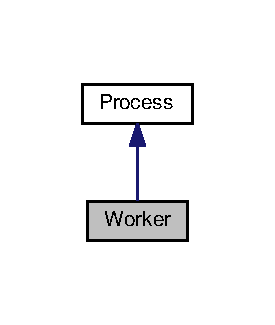
\includegraphics[width=132pt]{classWorker__coll__graph}
\end{center}
\end{figure}
\subsection*{Public Member Functions}
\begin{DoxyCompactItemize}
\item 
\hyperlink{classWorker_a3754817df06ffe220f7f0d903c78ccac}{Worker} ()
\item 
\hyperlink{classWorker_aa8e4543ef1e93fd9d884269ba30c5bfe}{$\sim$\-Worker} ()
\end{DoxyCompactItemize}
\subsection*{Additional Inherited Members}


\subsection{Constructor \& Destructor Documentation}
\hypertarget{classWorker_a3754817df06ffe220f7f0d903c78ccac}{\index{Worker@{Worker}!Worker@{Worker}}
\index{Worker@{Worker}!Worker@{Worker}}
\subsubsection[{Worker}]{\setlength{\rightskip}{0pt plus 5cm}Worker\-::\-Worker (
\begin{DoxyParamCaption}
{}
\end{DoxyParamCaption}
)\hspace{0.3cm}{\ttfamily [inline]}}}\label{classWorker_a3754817df06ffe220f7f0d903c78ccac}

\begin{DoxyCode}
26              \{
27     \}
\end{DoxyCode}
\hypertarget{classWorker_aa8e4543ef1e93fd9d884269ba30c5bfe}{\index{Worker@{Worker}!$\sim$\-Worker@{$\sim$\-Worker}}
\index{$\sim$\-Worker@{$\sim$\-Worker}!Worker@{Worker}}
\subsubsection[{$\sim$\-Worker}]{\setlength{\rightskip}{0pt plus 5cm}Worker\-::$\sim$\-Worker (
\begin{DoxyParamCaption}
{}
\end{DoxyParamCaption}
)\hspace{0.3cm}{\ttfamily [inline]}}}\label{classWorker_aa8e4543ef1e93fd9d884269ba30c5bfe}

\begin{DoxyCode}
30               \{
31     \}
\end{DoxyCode}


The documentation for this class was generated from the following file\-:\begin{DoxyCompactItemize}
\item 
worker/\hyperlink{worker_8hpp}{worker.\-hpp}\end{DoxyCompactItemize}

\chapter{File Documentation}
\hypertarget{comm_8hpp}{\section{comm/comm.hpp File Reference}
\label{comm_8hpp}\index{comm/comm.\-hpp@{comm/comm.\-hpp}}
}
{\ttfamily \#include $<$mpi.\-h$>$}\\*
Include dependency graph for comm.\-hpp\-:\nopagebreak
\begin{figure}[H]
\begin{center}
\leavevmode
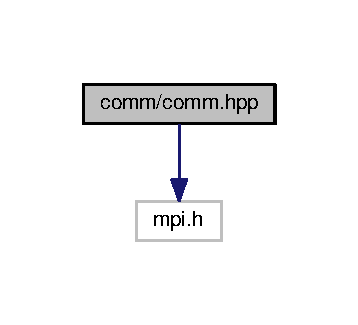
\includegraphics[width=172pt]{comm_8hpp__incl}
\end{center}
\end{figure}
This graph shows which files directly or indirectly include this file\-:\nopagebreak
\begin{figure}[H]
\begin{center}
\leavevmode
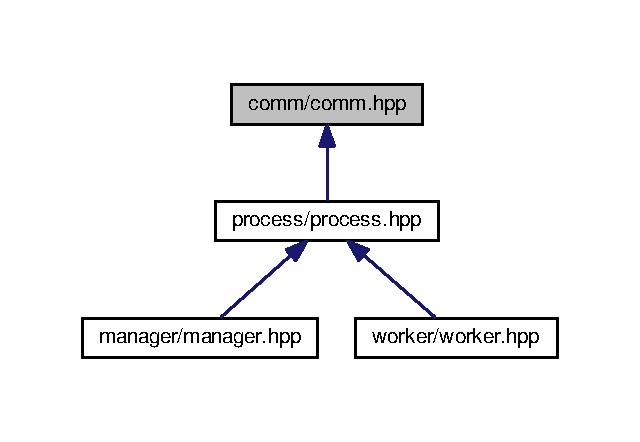
\includegraphics[width=307pt]{comm_8hpp__dep__incl}
\end{center}
\end{figure}
\subsection*{Classes}
\begin{DoxyCompactItemize}
\item 
class \hyperlink{classComm}{Comm}
\end{DoxyCompactItemize}


\subsection{Detailed Description}
Definition of communication structures and operations using M\-P\-I. Such definitions are used to support data exchanging between Anthill processing filters.

\begin{DoxyAuthor}{Author}
Bruno Rocha Coutinho \href{mailto:coutinho@dcc.ufmg.br}{\tt coutinho@dcc.\-ufmg.\-br} 

Rubens Emilio Alves Moreira \href{mailto:rubens@dcc.ufmg.br}{\tt rubens@dcc.\-ufmg.\-br}
\end{DoxyAuthor}
\begin{DoxyVersion}{Version}
x.\-y 
\end{DoxyVersion}

\hypertarget{manager_8cpp}{\section{manager/manager.cpp File Reference}
\label{manager_8cpp}\index{manager/manager.\-cpp@{manager/manager.\-cpp}}
}
{\ttfamily \#include $<$stdio.\-h$>$}\\*
{\ttfamily \#include $<$stdlib.\-h$>$}\\*
{\ttfamily \#include $<$mpi.\-h$>$}\\*
Include dependency graph for manager.\-cpp\-:
\nopagebreak
\begin{figure}[H]
\begin{center}
\leavevmode
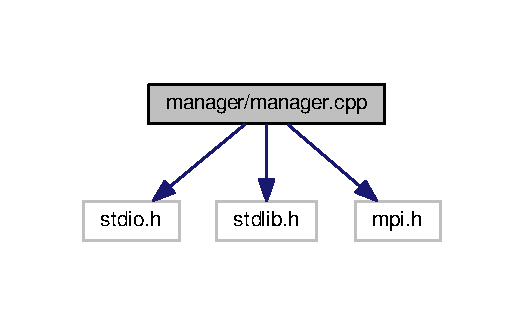
\includegraphics[width=251pt]{manager_8cpp__incl}
\end{center}
\end{figure}
\subsection*{Functions}
\begin{DoxyCompactItemize}
\item 
int \hyperlink{manager_8cpp_a0ddf1224851353fc92bfbff6f499fa97}{main} (int argc, char $\ast$argv\mbox{[}$\,$\mbox{]})
\end{DoxyCompactItemize}


\subsection{Function Documentation}
\hypertarget{manager_8cpp_a0ddf1224851353fc92bfbff6f499fa97}{\index{manager.\-cpp@{manager.\-cpp}!main@{main}}
\index{main@{main}!manager.cpp@{manager.\-cpp}}
\subsubsection[{main}]{\setlength{\rightskip}{0pt plus 5cm}int main (
\begin{DoxyParamCaption}
\item[{int}]{argc, }
\item[{char $\ast$}]{argv\mbox{[}$\,$\mbox{]}}
\end{DoxyParamCaption}
)}}\label{manager_8cpp_a0ddf1224851353fc92bfbff6f499fa97}

\begin{DoxyCode}
7                                  \{
8 
9     \textcolor{keywordtype}{int} SIZE = 10;
10     \textcolor{keywordtype}{double} a[SIZE][SIZE], b[SIZE], c[SIZE];
11     \textcolor{keywordtype}{int} i, j, row, numworkers;
12     MPI\_Status status;
13     MPI\_Comm workercomm;
14 
15     MPI::Init(argc, argv);
16     \textcolor{keywordflow}{if} (argc != 2)
17         printf(\textcolor{stringliteral}{"usage: %s <number of workers>\(\backslash\)n"}, argv[0]);
18     \textcolor{keywordflow}{else}
19         numworkers = atoi(argv[1]);
20     printf(\textcolor{stringliteral}{">>> %d WORKERS!\(\backslash\)n"}, numworkers);
21 
22     MPI\_Comm\_spawn(\textcolor{stringliteral}{"../worker/worker"}, MPI\_ARGV\_NULL, numworkers,
23                MPI\_INFO\_NULL,
24                0, MPI\_COMM\_SELF, &workercomm, MPI\_ERRCODES\_IGNORE );
25 
26     \textcolor{comment}{/* initialize a and b */}
27     
28     \textcolor{comment}{/* send b to each worker */}
29     
30     MPI\_Bcast( b, SIZE, MPI\_DOUBLE, MPI\_ROOT, workercomm );
31     
32     \textcolor{comment}{/* then normal manager code as before*/}
33 
34     MPI::Finalize();
35     \textcolor{keywordflow}{return} 0;
36 
37 \}
\end{DoxyCode}

\hypertarget{manager_8hpp}{\section{manager/manager.hpp File Reference}
\label{manager_8hpp}\index{manager/manager.\-hpp@{manager/manager.\-hpp}}
}
{\ttfamily \#include $<$xmlparser.\-hpp$>$}\\*
{\ttfamily \#include \char`\"{}../process/process.\-hpp\char`\"{}}\\*
Include dependency graph for manager.\-hpp\-:\nopagebreak
\begin{figure}[H]
\begin{center}
\leavevmode
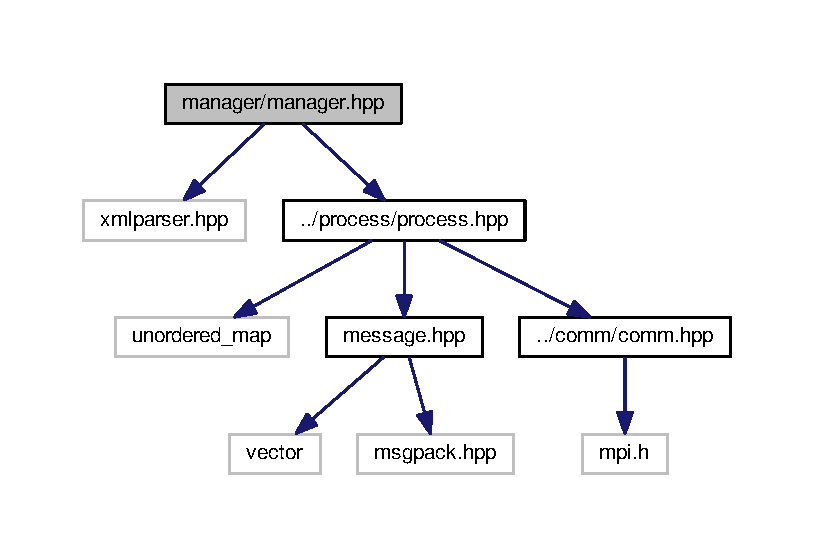
\includegraphics[width=350pt]{manager_8hpp__incl}
\end{center}
\end{figure}
\subsection*{Classes}
\begin{DoxyCompactItemize}
\item 
class \hyperlink{classManager}{Manager}
\end{DoxyCompactItemize}


\subsection{Detailed Description}
Set of operations designed to manage streams and filters, based on Anthill parallel processing model. The manager must\-:
\begin{DoxyItemize}
\item read up the configuration file -- config.\-xml;
\item set both the communication layout and process placement;
\item broadcast global configurations and parameters;
\item start the execution of loaded filters;
\item T\-O\-D\-O\-: treat user signals -- termination, global status, ...;
\item wait for the termination of entire process.
\end{DoxyItemize}

\begin{DoxyAuthor}{Author}
Bruno Rocha Coutinho \href{mailto:coutinho@dcc.ufmg.br}{\tt coutinho@dcc.\-ufmg.\-br} 

Rubens Emilio Alves Moreira \href{mailto:rubens@dcc.ufmg.br}{\tt rubens@dcc.\-ufmg.\-br}
\end{DoxyAuthor}
\begin{DoxyVersion}{Version}
x.\-y 
\end{DoxyVersion}

\hypertarget{message_8cpp}{\section{process/message.cpp File Reference}
\label{message_8cpp}\index{process/message.\-cpp@{process/message.\-cpp}}
}
{\ttfamily \#include $<$vector$>$}\\*
{\ttfamily \#include $<$iostream$>$}\\*
{\ttfamily \#include $<$msgpack.\-hpp$>$}\\*
Include dependency graph for message.\-cpp\-:\nopagebreak
\begin{figure}[H]
\begin{center}
\leavevmode
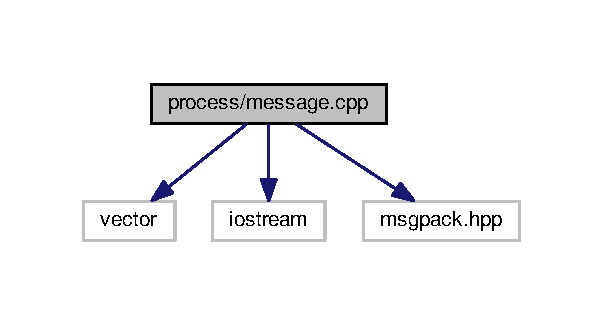
\includegraphics[width=289pt]{message_8cpp__incl}
\end{center}
\end{figure}
\subsection*{Functions}
\begin{DoxyCompactItemize}
\item 
int \hyperlink{message_8cpp_a840291bc02cba5474a4cb46a9b9566fe}{main} (void)
\end{DoxyCompactItemize}


\subsection{Function Documentation}
\hypertarget{message_8cpp_a840291bc02cba5474a4cb46a9b9566fe}{\index{message.\-cpp@{message.\-cpp}!main@{main}}
\index{main@{main}!message.cpp@{message.\-cpp}}
\subsubsection[{main}]{\setlength{\rightskip}{0pt plus 5cm}int main (
\begin{DoxyParamCaption}
\item[{void}]{}
\end{DoxyParamCaption}
)}}\label{message_8cpp_a840291bc02cba5474a4cb46a9b9566fe}

\begin{DoxyCode}
5                \{
6     \textcolor{comment}{// This is target object.}
7     std::vector<std::string> target;
8     target.push\_back(\textcolor{stringliteral}{"Hello,"});
9     target.push\_back(\textcolor{stringliteral}{"World!"});
10 
11     \textcolor{comment}{// Serialize it.}
12     msgpack::sbuffer sbuf;  \textcolor{comment}{// simple buffer}
13     msgpack::pack(&sbuf, target);
14 
15     \textcolor{comment}{// Deserialize the serialized data.}
16     msgpack::unpacked msg;    \textcolor{comment}{// includes memory pool and deserialized object}
17     msgpack::unpack(&msg, sbuf.data(), sbuf.size());
18     msgpack::object obj = msg.get();
19 
20     \textcolor{comment}{// Print the deserialized object to stdout.}
21     std::cout << obj << std::endl;    \textcolor{comment}{// ["Hello," "World!"]}
22 
23     \textcolor{comment}{// Convert the deserialized object to staticaly typed object.}
24     std::vector<std::string> result;
25     obj.convert(&result);
26 
27     \textcolor{comment}{// If the type is mismatched, it throws msgpack::type\_error.}
28     obj.as<\textcolor{keywordtype}{int}>();  \textcolor{comment}{// type is mismatched, msgpack::type\_error is thrown}
29 \}
\end{DoxyCode}

\hypertarget{message_8hpp}{\section{process/message.hpp File Reference}
\label{message_8hpp}\index{process/message.\-hpp@{process/message.\-hpp}}
}
{\ttfamily \#include $<$vector$>$}\\*
{\ttfamily \#include $<$msgpack.\-hpp$>$}\\*
Include dependency graph for message.\-hpp\-:\nopagebreak
\begin{figure}[H]
\begin{center}
\leavevmode
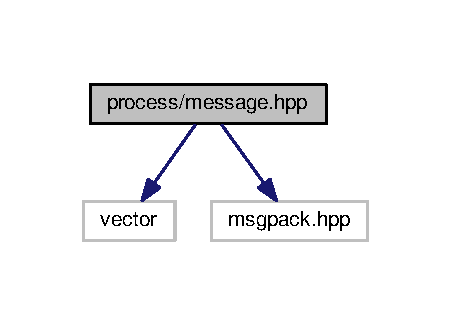
\includegraphics[width=216pt]{message_8hpp__incl}
\end{center}
\end{figure}
This graph shows which files directly or indirectly include this file\-:\nopagebreak
\begin{figure}[H]
\begin{center}
\leavevmode
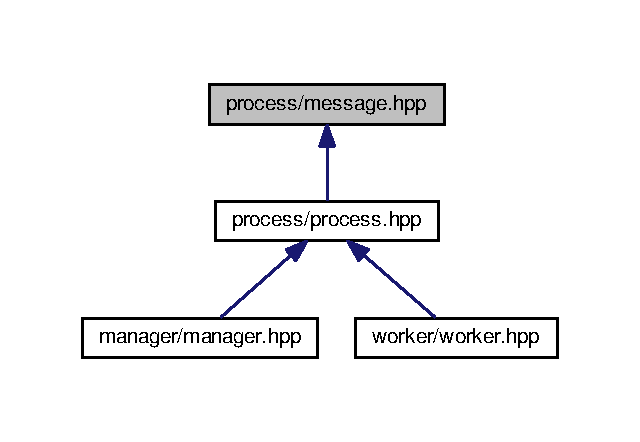
\includegraphics[width=307pt]{message_8hpp__dep__incl}
\end{center}
\end{figure}
\subsection*{Classes}
\begin{DoxyCompactItemize}
\item 
class \hyperlink{classMessage}{Message}
\end{DoxyCompactItemize}


\subsection{Detailed Description}
\hyperlink{classMessage}{Message} structure used by Anthill processes to exchange data. The encoding/decoding of C++ data structures is performed using the Msg\-Pack library, available at \href{http://msgpack.org/}{\tt http\-://msgpack.\-org/}

\begin{DoxyAuthor}{Author}
Bruno Rocha Coutinho \href{mailto:coutinho@dcc.ufmg.br}{\tt coutinho@dcc.\-ufmg.\-br} 

Rubens Emilio Alves Moreira \href{mailto:rubens@dcc.ufmg.br}{\tt rubens@dcc.\-ufmg.\-br}
\end{DoxyAuthor}
\begin{DoxyVersion}{Version}
x.\-y 
\end{DoxyVersion}

\hypertarget{process_8hpp}{\section{process/process.hpp File Reference}
\label{process_8hpp}\index{process/process.\-hpp@{process/process.\-hpp}}
}
{\ttfamily \#include $<$unordered\-\_\-map$>$}\\*
{\ttfamily \#include \char`\"{}message.\-hpp\char`\"{}}\\*
{\ttfamily \#include \char`\"{}../comm/comm.\-hpp\char`\"{}}\\*
Include dependency graph for process.\-hpp\-:\nopagebreak
\begin{figure}[H]
\begin{center}
\leavevmode
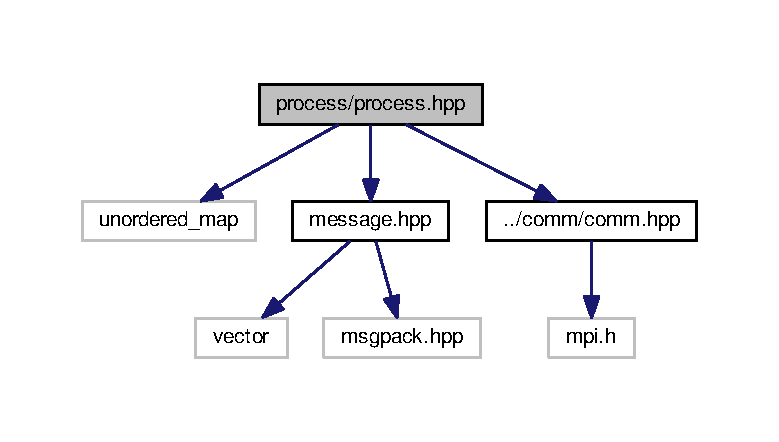
\includegraphics[width=350pt]{process_8hpp__incl}
\end{center}
\end{figure}
This graph shows which files directly or indirectly include this file\-:\nopagebreak
\begin{figure}[H]
\begin{center}
\leavevmode
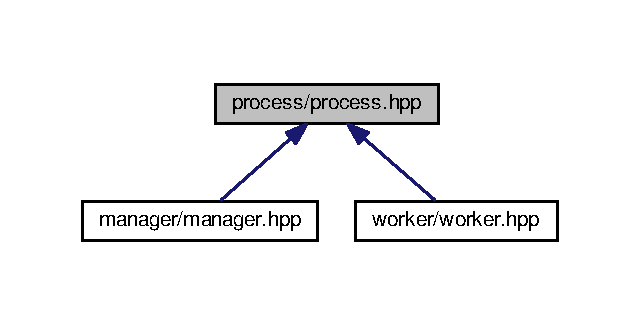
\includegraphics[width=307pt]{process_8hpp__dep__incl}
\end{center}
\end{figure}
\subsection*{Classes}
\begin{DoxyCompactItemize}
\item 
class \hyperlink{classProcess}{Process}
\end{DoxyCompactItemize}


\subsection{Detailed Description}
\hyperlink{classProcess}{Process} definition, supporting communication schemas. Classes inheriting this interface may act either as managers or workers in the Anthill parallel processing model.

\begin{DoxyAuthor}{Author}
Bruno Rocha Coutinho \href{mailto:coutinho@dcc.ufmg.br}{\tt coutinho@dcc.\-ufmg.\-br} 

Rubens Emilio Alves Moreira \href{mailto:rubens@dcc.ufmg.br}{\tt rubens@dcc.\-ufmg.\-br}
\end{DoxyAuthor}
\begin{DoxyVersion}{Version}
x.\-y 
\end{DoxyVersion}

\hypertarget{worker_8cpp}{\section{worker/worker.cpp File Reference}
\label{worker_8cpp}\index{worker/worker.\-cpp@{worker/worker.\-cpp}}
}
{\ttfamily \#include $<$mpi.\-h$>$}\\*
Include dependency graph for worker.\-cpp\-:\nopagebreak
\begin{figure}[H]
\begin{center}
\leavevmode
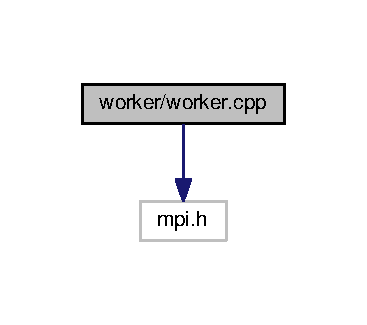
\includegraphics[width=176pt]{worker_8cpp__incl}
\end{center}
\end{figure}
\subsection*{Functions}
\begin{DoxyCompactItemize}
\item 
int \hyperlink{worker_8cpp_a0ddf1224851353fc92bfbff6f499fa97}{main} (int argc, char $\ast$argv\mbox{[}$\,$\mbox{]})
\end{DoxyCompactItemize}


\subsection{Function Documentation}
\hypertarget{worker_8cpp_a0ddf1224851353fc92bfbff6f499fa97}{\index{worker.\-cpp@{worker.\-cpp}!main@{main}}
\index{main@{main}!worker.cpp@{worker.\-cpp}}
\subsubsection[{main}]{\setlength{\rightskip}{0pt plus 5cm}int main (
\begin{DoxyParamCaption}
\item[{int}]{argc, }
\item[{char $\ast$}]{argv\mbox{[}$\,$\mbox{]}}
\end{DoxyParamCaption}
)}}\label{worker_8cpp_a0ddf1224851353fc92bfbff6f499fa97}

\begin{DoxyCode}
4                                  \{
5 
6     \textcolor{keywordtype}{int} SIZE = 10;
7     \textcolor{keywordtype}{int} numprocs, myrank;
8     \textcolor{keywordtype}{double} b[SIZE], c[SIZE];
9     \textcolor{keywordtype}{int} i, row;
10     \textcolor{keywordtype}{double} dotp;
11     MPI\_Status status;
12     MPI\_Comm parentcomm;
13 
14     MPI\_Init( &argc, &argv );
15     MPI\_Comm\_size( MPI\_COMM\_WORLD, &numprocs );
16     MPI\_Comm\_rank( MPI\_COMM\_WORLD, &myrank );
17 
18     printf(\textcolor{stringliteral}{"%d IS ALIVE!\(\backslash\)n"}, myrank);
19     MPI\_Comm\_get\_parent( &parentcomm );
20 
21     MPI\_Bcast( b, SIZE, MPI\_DOUBLE, 0, parentcomm );
22 
23     \textcolor{comment}{/* same as worker code from original matrix-vector multiply */}
24 
25     MPI\_Comm\_free( &parentcomm );
26     MPI::Finalize();
27     \textcolor{keywordflow}{return} 0;
28 
29 \}
\end{DoxyCode}

\hypertarget{worker_8hpp}{\section{worker/worker.hpp File Reference}
\label{worker_8hpp}\index{worker/worker.\-hpp@{worker/worker.\-hpp}}
}
{\ttfamily \#include $<$iostream$>$}\\*
{\ttfamily \#include \char`\"{}../process/process.\-hpp\char`\"{}}\\*
Include dependency graph for worker.\-hpp\-:\nopagebreak
\begin{figure}[H]
\begin{center}
\leavevmode
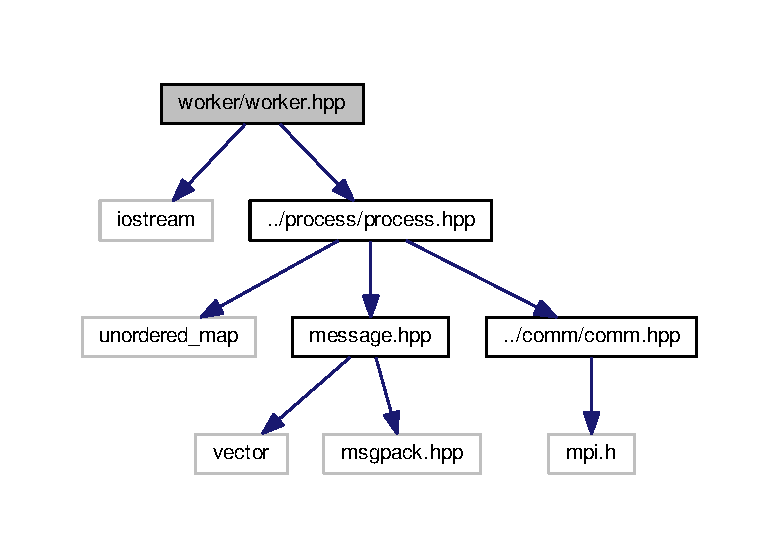
\includegraphics[width=350pt]{worker_8hpp__incl}
\end{center}
\end{figure}
\subsection*{Classes}
\begin{DoxyCompactItemize}
\item 
class \hyperlink{classWorker}{Worker}
\end{DoxyCompactItemize}


\subsection{Detailed Description}
\hyperlink{classWorker}{Worker} process definition, with virtual functions to be overridden by actual implementations. The user defined actions will be executed based on events -- be it either a message or a signal.

\hyperlink{classWorker}{Worker} processes must\-:
\begin{DoxyItemize}
\item define the virtual function {\ttfamily void Process()´;}
\item {\ttfamily instantiate}anthill\-::packer$<$tt$>$structures to send data;
\item instantiateanthill\-::unpacker$<$tt$>$structures to receive data;
\item callanthill\-::terminate()` to finish the execution.
\end{DoxyItemize}

\begin{DoxyAuthor}{Author}
Bruno Rocha Coutinho \href{mailto:coutinho@dcc.ufmg.br}{\tt coutinho@dcc.\-ufmg.\-br} 

Rubens Emilio Alves Moreira \href{mailto:rubens@dcc.ufmg.br}{\tt rubens@dcc.\-ufmg.\-br}
\end{DoxyAuthor}
\begin{DoxyVersion}{Version}
x.\-y 
\end{DoxyVersion}

%--- End generated contents ---

% Index
\newpage
\phantomsection
\addcontentsline{toc}{part}{Index}
\printindex

\end{document}
